% !TeX root = phd_thesis_Syromyatnikov.tex

\chapter{Структурный фазовый переход  в атомных цепочках Co на поверхности Cu(775)}
\label{chap:spt}

\blindfootnote{Результаты этой главы были опубликованы в работах A7, A8 из списка публикаций по теме диссертации.}
%\cite{Syromyatnikov:matlet:2016,Syromyatnikov:jetp-rus:2017}

\lipsum[1-3]

\section{Раздел 1}

\lipsum[4-5]

\begin{figure}
	\centering
	\tikzsetnextfilename{metropoliscircles}
	\begin{tikzpicture}[scale=1.5,every node/.append style={scale=1.5}]
	\tikzset{
		atom/.style={draw,ultra thin,circle,radius=1,minimum width=1cm,inner sep=0},
		%
		toplayer/.style=    {atom,fill=orange!1,draw=none},
		bottomlayer1/.style={atom,fill=orange!50,draw=none},
		bottomlayer2/.style={atom,fill=orange!70!black,draw=none},
		bottomlayer3/.style={atom,fill=orange!50!black,draw=none},
		%
		ag/.style={atom,ball color=DodgerBlue,minimum width=0.75cm}
	}
	
	\tikzmath{\atomswidth = 8;}
	
	\begin{scope}
	\clip (0.5, 1.5) rectangle (\atomswidth-0.5, -1.5);
	
	\begin{scope}[yshift=0.8657cm, xshift=0cm]
	
	\foreach \yshift/\nodestyle in {0/bottomlayer3, 0.578cm/bottomlayer2, -0.578cm/bottomlayer1}{
		\begin{scope}[yshift=\yshift]
		\foreach \y in {-5,...,5}{
			\foreach \x in {0,...,\atomswidth}{
				\tikzmath{if mod(\y, 2) == 0 then {\x = \x + 0.5;};}
				\node[\nodestyle] at (\x, \y*0.8657) {};
		}}
		\end{scope}
	}
	
	\foreach \y in {0,...,5}{
		\foreach \x in {0,...,\atomswidth}{
			\tikzmath{if mod(\y, 2) == 0 then {\x = \x + 0.5;};}
			\node[toplayer] at (\x, \y*0.8657) {};
	}}
	\end{scope}
	
	\fill[white,path fading=east](0.4,-1.6) rectangle (1.6,1.5);
	\fill[white,path fading=west](\atomswidth-1.5,-1.6) rectangle (\atomswidth-0.4,1.6);
	
	\end{scope}
	
	\foreach \x/\offset/\subscr in {1/1/i\vphantom{+}, 2/-1/i{+}1, 3/0/i{+}2, 4/1/i{+}3, 5/-1/i{+}4}{
		\node[ag] (ag\x) at (1+\x+\offset*0.125, 0) {};
		\fill[black,semitransparent] (1+\x+\offset*0.125,0) circle (0.05);
		
		\node[anchor=base,below=0.7cm] at (\x+1, 0) {\scriptsize $\offset$};
		\node[anchor=base,above=1.1cm,fill=none,inner sep=0.2] at (\x+1,0) {\scriptsize $\subscr$};
	}
	\foreach \x in {0,...,6}
	\draw (\x+1,-0.1) -- ++(0,0.2);
	\foreach \x in {0,6}{
		\node[anchor=base,below=0.7cm] at (\x+1, 0) {\scriptsize $\cdots$};
		\node[anchor=base,above=1.1cm,inner sep=0.2] at (\x+1,0) {\scriptsize $\cdots$};
	}
	
	\draw[] (0.25,0) -- (7.75,0);
	\node[below=0.7cm] at (0,0) {\scriptsize $s_i =$};
	
	\draw[white] (0,-1.5) circle (0.01); % fixes margin below
	\end{tikzpicture}
	\caption{Графическое представление способа расчета параметра порядка. Синие шарики --- атомы цепочки, оранжевые круги --- нижняя терраса подложки, белые --- верхняя терраса подложки.}
	\label{fig:metropoliscircles}
\end{figure}

\lipsum[6-7]

\section{Раздел 2}
\lipsum[11-14]

\begin{figure}
	\centering
	\tikzsetnextfilename{differentdE}
	\begin{tikzpicture}
	\pgfplotsset{
		every axis/.append style={
			width=0.5\linewidth, height=8cm, no markers, enlargelimits=0, xmin=0,
			% cycle list={tabred,taborange,tabgreen,tabblue,black},
			cycle list={black,tabblue,tabgreen,taborange,tabred},
			% cycle list={tabblue,tabgreen,taborange,tabred},
		},
		every axis plot/.append style={very thick, mark=none,},
		every axis legend/.append style={
			draw=none,cells={anchor=east},at={(0.98,0.4)},anchor=east,outer xsep=0,
		},
	}
	
	\pgfplotstableread[col sep=comma]{fig/spt/dE=10-etas.csv}\Eetas
	\pgfplotstableread[col sep=comma]{fig/spt/dE=10-detas.csv}\Edetas
	\pgfplotstableread[col sep=comma]{fig/spt/len=64-etas.csv}\Letas
	\pgfplotstableread[col sep=comma]{fig/spt/len=64-detas.csv}\Ldetas
	
	\begin{axis}[
	name=A,
	yticklabel=\tickprint{fixed,fixed zerofill,precision=1},
	xticklabels=\empty,ymin=-0.02,xmax=185,ymax=1.02,
	ylabel={$\eta$}
	]
	\addplot table[x=T,y=e16]{\Eetas};
	% \addplot table[x=T,y=e32]{\Eetas};
	\addplot table[x=T,y=e48]{\Eetas};
	% \addplot table[x=T,y=e64]{\Eetas};
	% \addplot table[x=T,y=e96]{\Eetas};
	\addplot table[x=T,y=e128]{\Eetas};
	% \addplot table[x=T,y=e256]{\Eetas};
	\addplot table[x=T,y=e512]{\Eetas};
	\end{axis}
	
	\begin{axis}[
	name=B, at=(A.south), anchor=north, yshift=-0.2cm,
	yticklabel=\tickprint{fixed,fixed zerofill,precision=2},
	xmax=185,ymax=0.032,
	ylabel={$-\od{\eta}{T}$, К$^{-1}$}, xlabel={$T$, К},
	legend style={name=legB},
	]
	\addplot table[x=T,y=de16]{\Edetas}; \addlegendentry{16 атомов};
	% \addplot table[x=T,y=de32]{\Edetas}; \addlegendentry{32 атома};
	\addplot table[x=T,y=de48]{\Edetas}; \addlegendentry{48 атомов};
	% \addplot table[x=T,y=de64]{\Edetas}; \addlegendentry{64 атома};
	% \addplot table[x=T,y=de96]{\Edetas}; \addlegendentry{96 атомов};
	\addplot table[x=T,y=de128]{\Edetas}; \addlegendentry{128 атомов};
	% \addplot table[x=T,y=de256]{\Edetas}; \addlegendentry{256 атомов};
	\addplot table[x=T,y=de512]{\Edetas}; \addlegendentry{512 атомов};
	\end{axis}
	
	\begin{axis}[
	name=C, at=(A.east), anchor=west, xshift=0.8cm,
	xticklabels=\empty, yticklabels=\empty, 
	ymin=-0.02, xmax=400, ymax=1.02,
	cycle list={tabblue,tabgreen,taborange,tabred},
	]
	\node at (310,0.2) {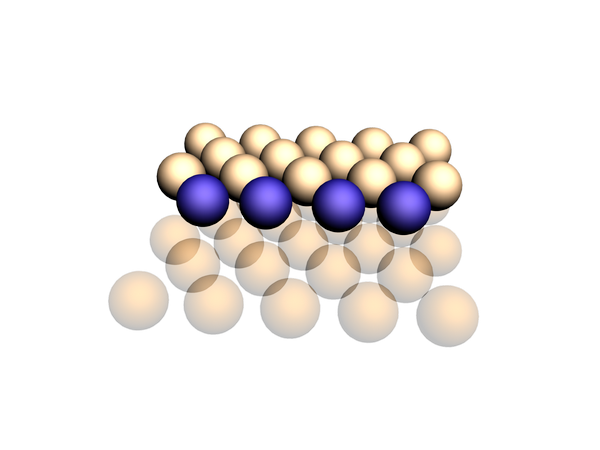
\includegraphics[width=0.25\linewidth]{fig/spt/none.png}};
	\node at (130,0.65) {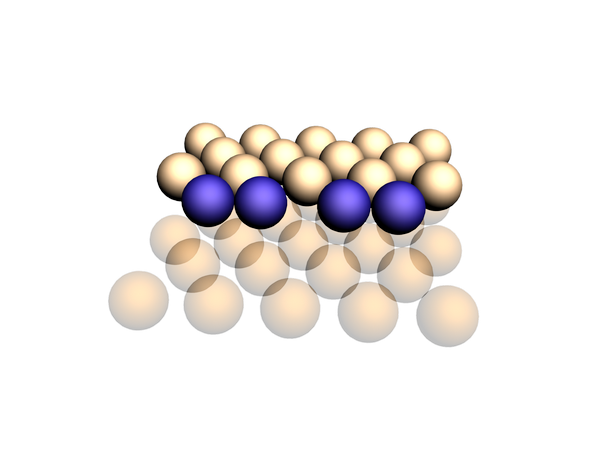
\includegraphics[width=0.25\linewidth]{fig/spt/dipoles-noarrows.png}};
	
	\addplot table[x=T,y=e4]{\Letas};
	\addplot table[x=T,y=e10]{\Letas};
	\addplot table[x=T,y=e16]{\Letas};
	\addplot table[x=T,y=e64]{\Letas};
	
	\draw[thin,tabred,dashed] (225,0) -- ++(0,1);
	\end{axis}
	
	\begin{axis}[
	name=D, at=(C.south), anchor=north, yshift=-0.2cm,
	yticklabels=\empty, xmax=400, ymax=0.032,
	xlabel={$T$, К},
	cycle list={tabblue,tabgreen,taborange,tabred},
	legend style={name=legD},
	]
	\addplot table[x=T,y=de4]{\Ldetas}; \addlegendentry{4 мэВ};
	\addplot table[x=T,y=de10]{\Ldetas}; \addlegendentry{10 мэВ};
	\addplot table[x=T,y=de16]{\Ldetas}; \addlegendentry{16 мэВ};
	\addplot table[x=T,y=de64]{\Ldetas}; \addlegendentry{64 мэВ};
	
	\draw[thin,tabred,dashed] (225,0) -- ++(0,0.04);
	\end{axis}
	
	\tikzset{tag/.style={below left=0.5cm}}
	\node[tag] at (A.north east) {а};
	\node[tag] at (B.north east) {б};
	\node[tag] at (C.north east) {в};
	\node[tag] at (D.north east) {г};
	
	\node[above left] at (legB.north east) {Длина цепочки};
	\node[above left] at (legD.north east) {$\Delta E$};
	\end{tikzpicture}
	\caption{Зависимости параметра порядка $\eta$ и его производной по температуре с обратным знаком $-\od{\eta}{T}$ от температуры для (а, б) цепочек различной длины с $\Delta E=10$~мэВ и (в, г) цепочек длиной 64 атома с разными значениями энергии димеризации $\Delta E$. Подписи к кривым общие для графиков (а) и (б), и (в) и (г).
	Вертикальная пунктирная линия на рисунках (в, г) соответствует температуре структурного фазового перехода для цепочки длиной 64 атома с $\Delta E = 64$~мэВ. Для наглядности слева и справа от нее на рисунке (в) схематически нарисована цепочка до и после структурного фазового перехода.
	}
	\label{fig:etasv2}
\end{figure}
